% This is samplepaper.tex, a sample chapter demonstrating the
% LLNCS macro package for Springer Computer Science proceedings;
% Version 2.21 of 2022/01/12
%
\documentclass[runningheads]{llncs}
%
\usepackage[T1]{fontenc}
% T1 fonts will be used to generate the final print and online PDFs,
% so please use T1 fonts in your manuscript whenever possible.
% Other font encondings may result in incorrect characters.
%
\usepackage{graphicx}
\usepackage{cite}
\usepackage{amsmath,amssymb,amsfonts}
\usepackage{booktabs} 
\usepackage{graphicx}
\usepackage{textcomp}
\usepackage{xcolor}
\usepackage{graphics}
\usepackage{algorithm}
\usepackage{algpseudocode}
% Used for displaying a sample figure. If possible, figure files should
% be included in EPS format.
%
% If you use the hyperref package, please uncomment the following two lines
% to display URLs in blue roman font according to Springer's eBook style:
%\usepackage{color}
%\renewcommand\UrlFont{\color{blue}\rmfamily}
%\urlstyle{rm}
%
\begin{document}
%
\title{Streamlined Data Pipeline for Real-Time Threat Detection and Model Inference}
%
\titlerunning{Real-Time Threat Detection Pipeline}
% If the paper title is too long for the running head, you can set
% an abbreviated paper title here
%
% \author{Rajkanwar Singh\inst{1}\orcidID{0009-0009-4267-7398} \and
% Aravindan V\inst{1}\orcidID{0009-0006-3078-0986} \and
% Sanket Mishra\inst{1}\orcidID{0000-0002-3193-8160}}
%
% \authorrunning{Singh R. et al.}
% First names are abbreviated in the running head.
% If there are more than two authors, 'et al.' is used.
%
% \institute{School of Computer Science and Engineering, VIT-AP University, Amaravati, India
% \email{sanketmishra@live.com}\\
% }
%
\maketitle              % typeset the header of the contribution
%
\begin{abstract}
Real-time threat detection in streaming data is crucial yet challenging due to varying data volumes and speeds. This paper presents an architecture designed to manage large-scale, high-speed data streams using deep learning and machine learning models. The system utilizes Apache Kafka for high-throughput data transfer and a publish-subscribe model to facilitate continuous threat detection. Various machine learning techniques, including XGBoost, Random Forest, and LightGBM, are evaluated to identify the best model for classification. The ExtraTrees model achieves exceptional performance with accuracy, precision, recall, and F1 score all reaching 99\% using the SensorNetGuard dataset within this architecture. The PyFlink framework, with its parallel processing capabilities, supports real-time training and adaptation of these models. The system calculates prediction metrics every 2,000 data points, ensuring efficient and accurate real-time threat detection. 

\keywords{Malicious Node  \and Big Data Analytics \and Online Machine Learning \and Internet of Things}
\end{abstract}
%
%
%

\section{Introduction}
\label{sec:Intro}

Cyberattacks have increased as the digital landscape expands, and malicious actors employ more sophisticated tactics. Identifying and mitigating these threats is a high priority. The proliferation of connected devices and the increasing dependence on online platforms create more opportunities for cybercriminals to exploit vulnerabilities. In addition, the sophistication of attacks has grown, making them harder to detect and defend against. Intrusion detection systems (IDSs) must continuously improve their ability to detect new types of attack.

The surge in Internet of Things (IoT) devices and sensors generates large amounts of data that can contain threats or anomalies that require attention. Detecting these anomalies is essential in real-life applications, such as identifying fraudulent financial transactions, fake calls, network intrusions, and healthcare care anomalies. Such detection provides insights that might otherwise be overlooked. In a streaming environment, storing and processing data can be unfeasible due to high I/O usage or the need for real-time analysis.

Real-time streaming data processing demands high throughput, low latency, fault tolerance, and highly scalable platforms. Computing platforms are required to handle batch and stream processing, while streaming architectures must efficiently transmit, consume, and process data.

This study introduces a high-throughput architecture that combines deep learning and machine learning models to detect malicious nodes in real-time IoT data streams. The design utilizes a publish-subscribe mechanism, wherein data is posted to a Kafka topic observed by the consumer. PyFlink acts as the consumer, employing the data for threat classification and detection, and functions as the processor within Kafka's system framework. Various machine learning and deep learning models are utilized to select features, competing to produce the best set of features. The outputs from the first model to the final version are published in Kafka. This method aims to provide the quickest results, regardless of the dataset fed into the system. The proposed architecture selects the optimal models, guaranteeing reliable results even with changes in dataset. Identifies a feature set that can easily be adjusted to changes in data. Using this feature set, a PyFlink job trains models like Random Forest, XGBoost, and LightGBM; predictions are then produced using the model with the best performance. With PyFlink, a distributed computing and stream processing framework, these models are trained efficiently, enabling continuous model updates and retraining as needed. This allows the architecture to adapt and retain accuracy as the data evolve.

\subsection{Organisation}
This paper is organised as follows. Section \ref{sec:Intro} is the introductory section while Section \ref{sec:Literature-Review} throws light on the research done in this field previously by other researchers. Section \ref{sec:Methodology} explains various components used, the architecture and their functioning. Section \ref{sec:Results-and-Discussion} discusses the application of the architecture to the SensorNetGuard data set \cite{b3}. The last section of the paper is the summary of the work and also the future scope of the study.

\section{Literature Review}
\label{sec:Literature-Review}

Ibra Him \cite{b4} in his paper explores the integration of Artificial Intelligence (AI) and Machine Learning (ML) into real-time threat intelligence frameworks to improve cybersecurity. The paper discusses how AI and ML can analyze vast data sources in real time, identify patterns, and detect anomalies indicative of potential threats. The research also examines the integration of AI-driven analytics with existing security infrastructure, such as Security Information and Event Management (SIEM) systems, to provide contextualized insights and prioritized alerts. The study also evaluates the performance of AI algorithms through prototype systems and simulations, comparing them with traditional methods to quantify their effectiveness and scalability. Surianarayanan et. al. \cite{b2}  propose a high-throughput streaming architecture for real-time anomaly detection using machine learning algorithms. Their architecture leverages Apache Kafka for data ingestion and Random Forest (RF) for anomaly detection. It achieves near-zero latency and high accuracy (up to 98. 6\%) in single- and distributed node configurations. However, the data are not publicly available. Using random forest (RF) and k-means clustering techniques in the CIC-IDS 2018 dataset, Mudgal and Bhalla \cite{b5} achieved a precision of 99. 66\% and managed to reduce latency by 30\% with the implementation of their Honeypot Intelligence-enabled intrusion detection system. Their study presents the Honeypot intelligence system's deployment on Flink. The study conducted by Deepthi et. al. \cite{b6} introduces a Flexible Real-Time Traffic Stream Processing System (FRTSPS), crafted to manage the intricacies of real-time traffic data streams. This system's architecture is built on the Lambda structure and leverages Apache Flink to process both historical and real-time data. Their results showcase a 25\% decrease in latency. Additionally, the proposed system boasts higher Events/sec per CPU core and per Data Size compared to Apache Spark and Apache Storm. An additional study introduces a modular and horizontally scalable IDS architecture suitable for data capture, storage, and analysis in real-time or near real-time within a 1 Gbps network environment \cite{b7}. The architecture consists of modules for packet capture, queueing, storage, and analysis. The paper elaborates on the experimental evaluation of this architecture, focusing on performance benchmarks and technology choices such as tcpdump, Apache Kafka, HDFS, and Apache Spark. Kajiura and Nakamura \cite{b8} analyze the performance of a distributed processing framework for machine learning-based network intrusion detection systems (NIDS). They deploy five classifiers (Decision Tree, Random Forest, Naive Bayes, SVM, and kNN) and measure their throughput and latency. Their findings show significant differences in classifier performance and processing speed, with Decision Tree and Naive Bayes obtaining the highest throughput. The study identifies bottlenecks within the framework, especially in the Zeek, Logstash, and Elasticsearch components, and suggests that the selection of suitable machine learning algorithms can reduce system load while maintaining high classifier performance. Atbib et al. \cite{b9} propose a Distributed Intrusion Detection System tailored for streaming data in IoT environments. The IDS is implemented within a Fog computing architecture using Apache Spark and various machine learning algorithms, with the aim of providing real-time intrusion detection by analyzing data from the NF-ToN-IoT-v2 dataset. The proposed architecture includes three layers: IoT nodes, Fog, and Cloud. The models deployed are Decision Tree (86\% accuracy), Random Forest (87\% accuracy), Support Vector Machine (60\% accuracy), Logistic Regression (73\% accuracy) and Naive Bayes (49\% accuracy). Decision Tree and Random Forest outperform other models in all evaluated metrics. Jemili et al. \cite{b10} tackle the challenges posed to traditional intrusion detection methods by evolving cyber threats. They present a hybrid intrusion detection model that integrates Random Forest, XGBoost, and decision trees, leveraging ensemble learning to increase accuracy, adaptability, and robustness. The study tests the model using datasets such as N-BaIoT, NSL-KDD, and CICIDS2017, achieving accuracy rates that exceed 97\%. The results emphasize the superiority of the hybrid approach in detecting intrusions in Big Data environments. Ashraf et al. \cite{b11} focus on developing an IoT-based smart cybersecurity framework for intrusion detection on the Internet of Drones (IoD). The paper discusses the integration of machine learning (ML) and deep learning (DL) techniques to improve the security of drone networks. Their research addresses privacy and security challenges in IoD, suggesting a system that effectively identifies cyberattacks using B-LSTM and LSTM models. This framework, tested on the CICIDS2017 and KDDCup 99 datasets, demonstrates high precision (89.10\% and 90.16\%), accuracy (91.00 and 91.36\%), recall (81.13\% and 90.11\%), and F-measure scores (88.11\% and 90.19\%).
\section{Methodology}
\label{sec:Methodology}

\begin{figure}[htbp]
\centerline{\includegraphics[width=\linewidth]{images/DFD.png}}
\caption{BARS Architecture}
\label{fig:DFD}
\end{figure}

\subsection{Tools and Technologies Used}
\subsubsection{Flask API}
Flask API hosted on port 5001 (mapped to 5000 on system) to receive sensor data from HTTP POST requests and send those data to a Kafka topic. It also maintains a delivery report function that logs whether Kafka message delivery was successful or not. Polling and Flushing are used to ensure that messages are sent by polling the producer and flushing the queue. The message key is a JSON string that contains the id of the data. The message value is the JSON string representation of the entire data.

\subsubsection{Apache Kafka}
Apache Kafka is an open source distributed streaming platform that offers highly scalable and fault-tolerant data processing capabilities for real-time data processing, alerting, and reporting. \cite{b12}
Kafka is used in the work as a message broker and serves as the central nervous system of the framework. It provides a pub-sub model allowing various sources of inflow and outflow to various engines/frameworks, while also having higher throughput. \cite{b13}

\subsubsection{Apache Flink}
Apache Flink unifies diverse data processing applications in a single execution model, allowing real-time analytics, continuous data pipelines, historic data processing, and iterative algorithms \cite{b14}.

\subsubsection{PostegreSQL}
The PostegreSQL database is used to maintain a record of data received and predictions on data to be used as a fallback in case of Kafka failure. 

\subsubsection{Docker}
Docker, a Platform as a Service (PaaS) uses OS-level virtualization to deliver software in containers. Each container is built using an image and each of the containers is isolated \cite{b15}. Docker compose has been used to launch all containers in the same stack and hosted on the same network by means of a YAML file. Docker is used to orchestrate containerized applications that provide container flexibility, consistency, and user-friendliness. Fig. \ref{fig:docker-compose} depicts a screenshot of the Docker stack (with multiple containers) used in this work. 

\subsubsection{Feature Selection}
Two deep learning methods for feature selection were long-short-term memory (LSTM) networks and Deep Neural Networks (DNN). 33,441 trainable parameters were split across two LSTM layers and one dense layer in the LSTM model. The DNN model included six layers and 12,673 trainable parameters.
These models were optimized using Particle Swarm Optimization (PSO), which is renowned for its quick convergence. Furthermore, LightGBM and other machine learning models were used for feature extraction, and both PSO and Genetic Algorithms (GA) were used for optimization.Both PSO and GA are wrapper functions. 
A total of four feature sets were generated. To optimize the architecture, priority was given to the feature set that was produced first. This was achieved by creating a race condition through the use of multithreading techniques.

\subsubsection{Classifiers}
Batch mode on PyFlink was used to train five classifiers: Random Forest, Gradient Boosting, XGBoost, LightGBM, and Extra Trees. After that, the best model from this group of classifiers is chosen to predict the streaming data. 

\begin{figure}[htbp]
\centerline{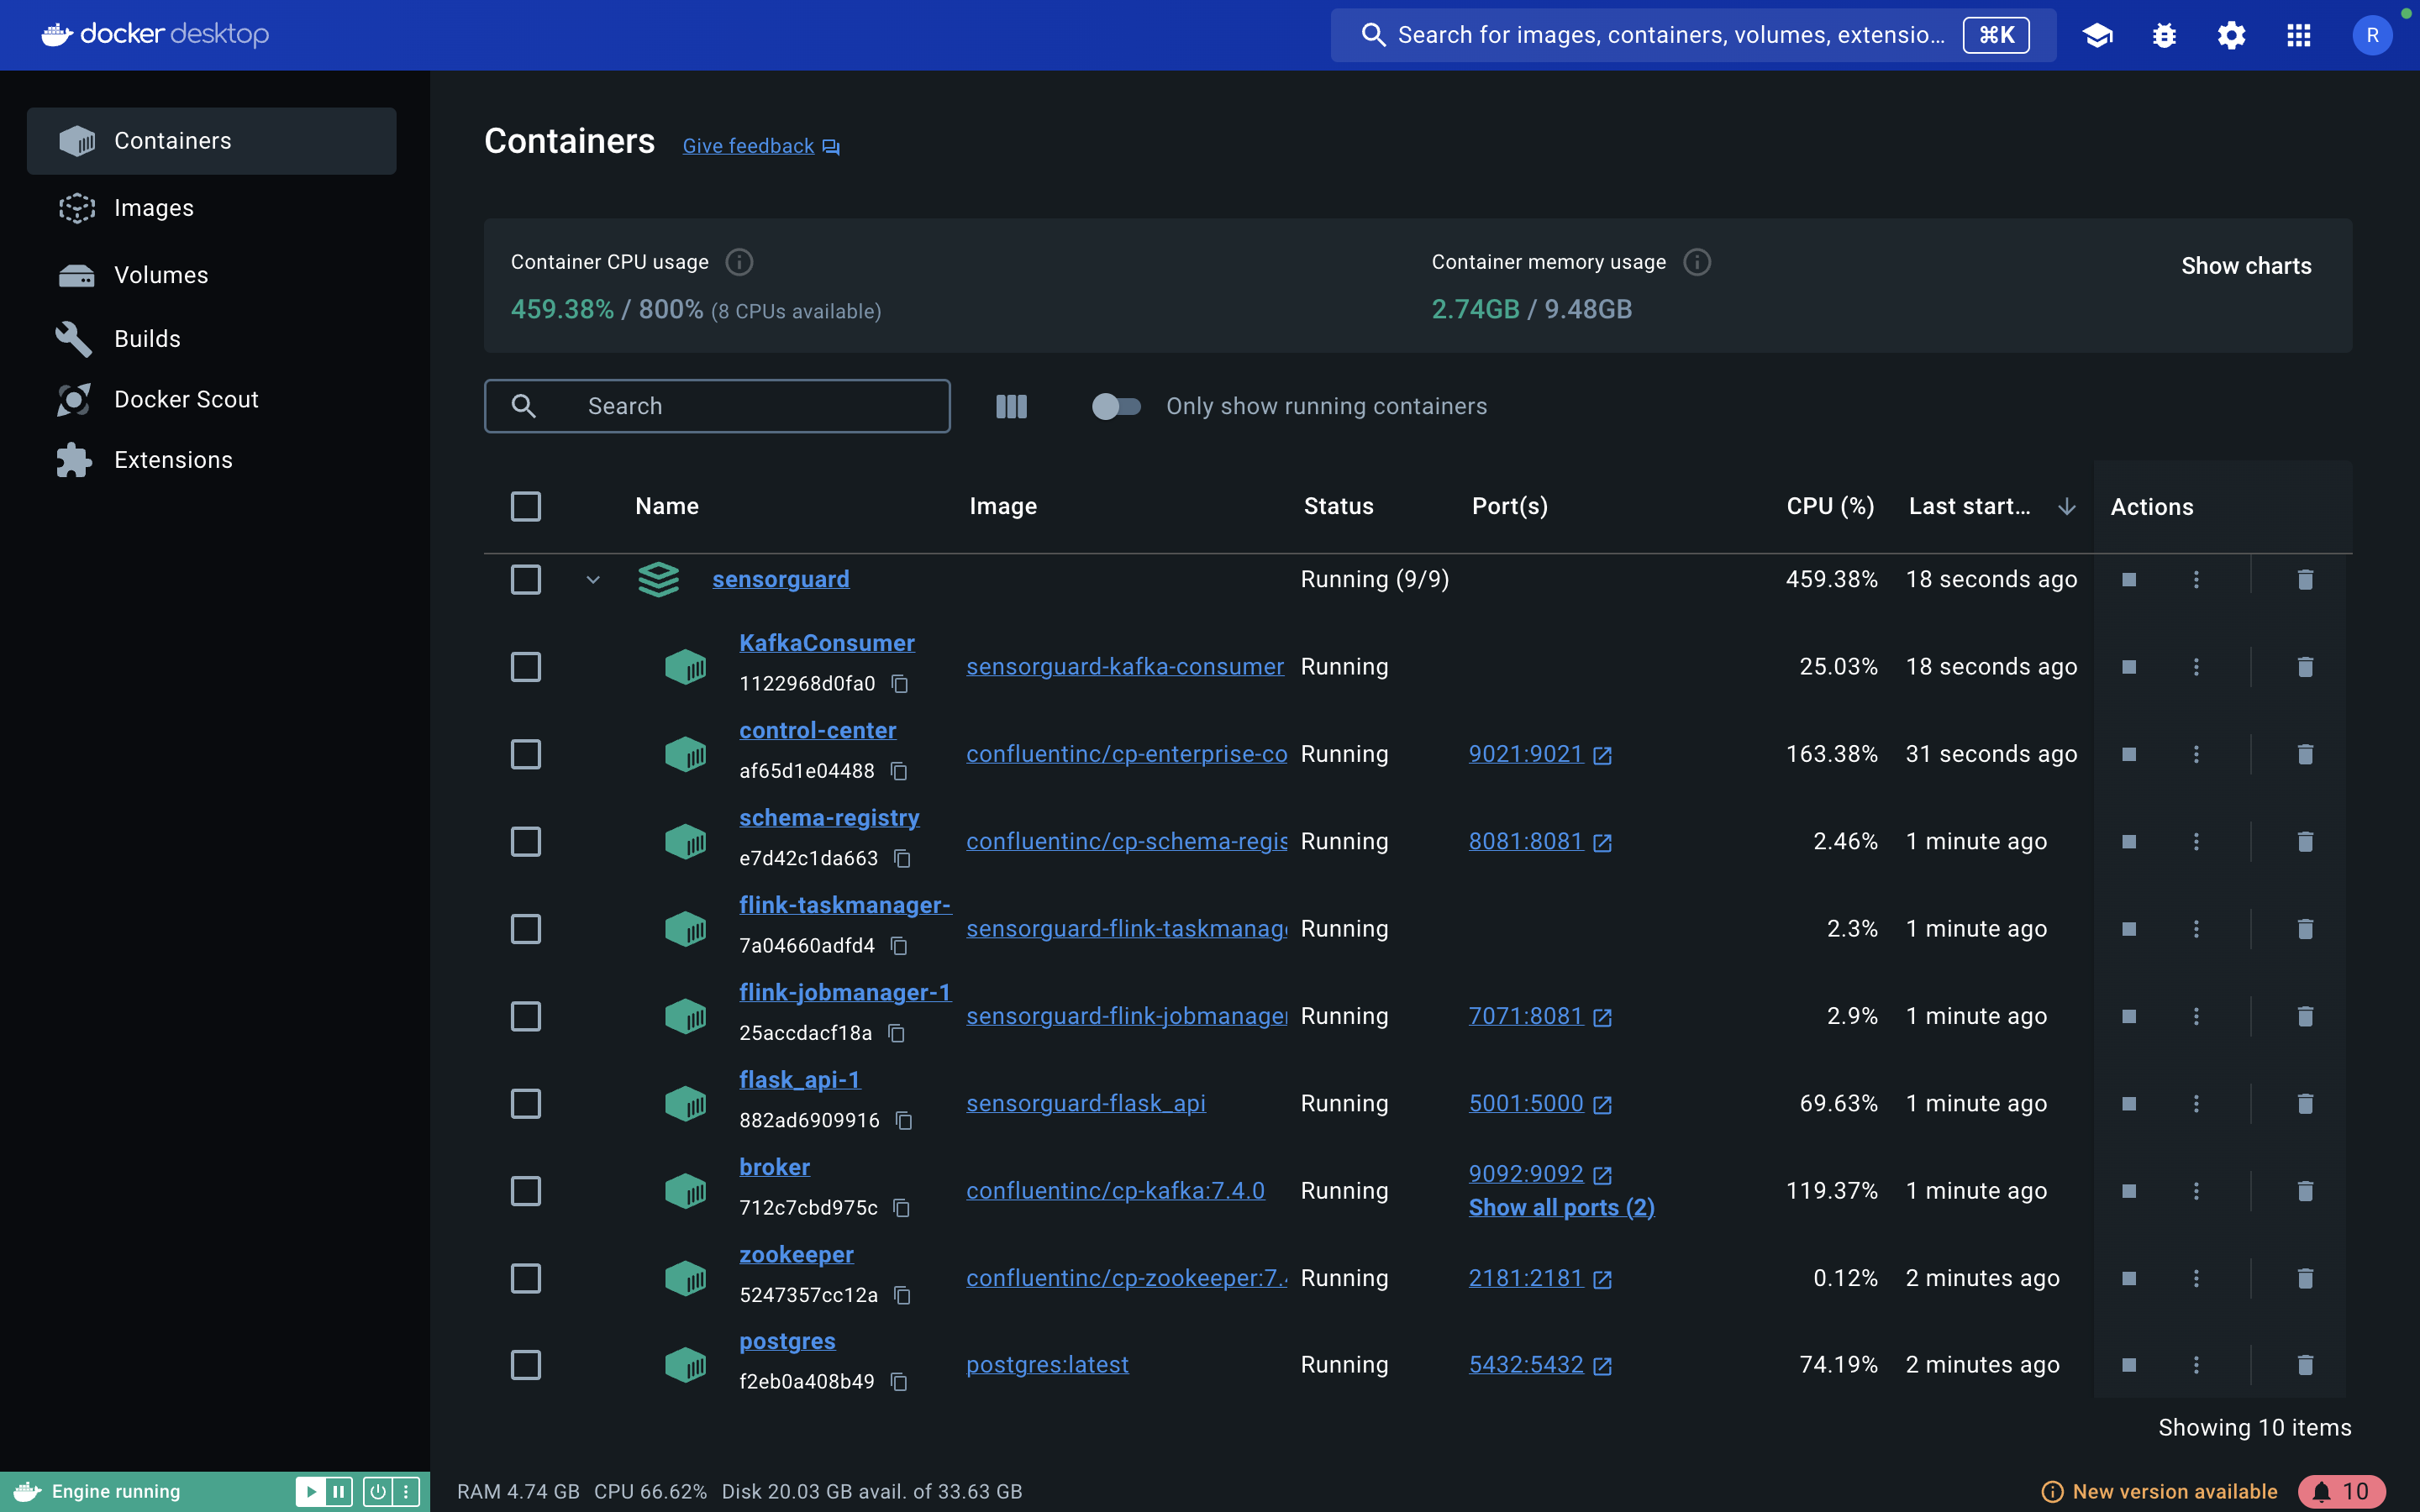
\includegraphics[width=\linewidth]{images/docker-compose.png}}
\caption{A screenshot of pipeline components in Docker}
\label{fig:docker-compose}
\end{figure}

% \begin{figure*}[!t]
%     \centering
%     \begin{minipage}{1\textwidth}
%         \scriptsize  % Adjust font size here
%         \begin{algorithm}[H]
%             \caption{Resample Data with Target Count}
%             \label{resampling_algo}

%             \begin{algorithmic}[1]
%             \State \textbf{Input:} $df$: DataFrame with data to be resampled
%             \State \textbf{Input:} $class\_column$: Name of the column with class labels
%             \State $class\_counts \gets df[class\_column].\text{value\_counts}()$
%             \State $majority\_class \gets \text{max}(class\_counts)$
%             \State $minority\_class \gets \text{min}(class\_counts)$
%             \State $target\_count \gets \frac{majority\_class + minority\_class}{2}$  \Comment{Target count for balancing}
%             \State $resampled\_dfs \gets []$  \Comment{List to store resampled DataFrames}
            
%             \For{each $(class\_value, count)$ in $class\_counts$}
%                 \State $class\_df \gets df[df[class\_column] == class\_value]$
                
%                 \If{$count < target\_count$}
%                     \State $resampled\_df \gets \text{resample}(class\_df, \text{replace=True}, \text{n\_samples=target\_count}, \text{random\_state=42})$
%                 \ElsIf{$count > target\_count$}
%                     \State $resampled\_df \gets \text{resample}(class\_df, \text{replace=False}, \text{n\_samples=target\_count}, \text{random\_state=42})$
%                 \Else
%                     \State $resampled\_df \gets class\_df$
%                 \EndIf
                
%                 \State $resampled\_dfs.\text{append}(resampled\_df)$
%             \EndFor
            
%             \State $resampled\_df \gets \text{pd.concat}(resampled\_dfs)$
%             \State \textbf{Output:} $resampled\_df$
%             \end{algorithmic}
%         \end{algorithm}
%     \end{minipage}
% \end{figure*}
\begin{figure*}[!t]
    \centering
    \begin{minipage}{0.85\textwidth}  % Slightly narrower minipage for Springer format
        \scriptsize  % Adjust font size here
        \begin{algorithm}[H]
            \caption{Resample Data with Target Count}
            \label{resampling_algo}

            \begin{algorithmic}[1]
            \State \textbf{Input:} $df$: DataFrame with data to be resampled
            \State \textbf{Input:} $class\_column$: Name of the column with class labels
            \State $class\_counts \gets df[class\_column].\text{value\_counts}()$
            \State $majority\_class \gets \text{max}(class\_counts)$
            \State $minority\_class \gets \text{min}(class\_counts)$
            \State $target\_count \gets \frac{majority\_class + minority\_class}{2}$ 
            \Comment{Target count for balancing}
            \State $resampled\_dfs \gets []$  \Comment{List to store resampled DataFrames}
            
            \For{each $(class\_value, count)$ in $class\_counts$}
                \State $class\_df \gets df[df[class\_column] == class\_value]$
                
                \If{$count < target\_count$}
                    \State $resampled\_df \gets \text{resample}(class\_df, \text{replace=True},$
                    \Statex \hspace{10em} $\text{n\_samples=target\_count}, \text{random\_state=42})$
                \ElsIf{$count > target\_count$}
                    \State $resampled\_df \gets \text{resample}(class\_df, \text{replace=False},$
                    \Statex \hspace{10em} $\text{n\_samples=target\_count}, \text{random\_state=42})$
                \Else
                    \State $resampled\_df \gets class\_df$
                \EndIf
                
                \State $resampled\_dfs.\text{append}(resampled\_df)$
            \EndFor
            
            \State $resampled\_df \gets \text{pd.concat}(resampled\_dfs)$
            \State \textbf{Output:} $resampled\_df$
            \end{algorithmic}
        \end{algorithm}
    \end{minipage}
\end{figure*}

\subsection{Integration and Flow}
Apache Flink and Apache Kafka together create a complete set of tools for real-time data processing and analysis, improving decision-making and flexibility \cite{b16}.
Fig. \ref{fig:DFD} depicts the flow of data in the pipeline.
Raw data is collected via a REST API and produced to Kafka topic/s as per the API endpoint, i.e., different topic for different API endpoint. All of these topics are subscribed to by Flink sinks in various jobs. The first job performs feature extraction by way of Deep Learning frameworks namely- LSTM, DNN and machine learning algorithm (LightGBM) and are optimised with  algorithms namely- Particle Swarm Optimization (PSO) and Genetic Algorithm.These algorithms run parallelly using multi threading. The extracted features are posted on various Kafka topics. A race condition is created to wait for the fastest algorithm to post its features, which are then posted to a final topic. LSTM optimised with PSO has consistently been the first to publish the results on the topic\footnote{The results of other methods have been explored but have not been discussed due to page limitations}. This topic is subscribed to by the next job for model training. The model training job ingests features and data from relevant Kafka topics and trains five machine learning algorithms on these data. Before training, the dataframe is passed through a customised resampler as highlighted in Algorithm \ref{resampling_algo}. A comparison of the original and resampled class distributions can be seen in Fig \ref{fig:resamp}. All trained models are serialized as pickle files (.pkl) and stored in a shared volume between the Flink Task-Manager and the Job-Manager. This job also saves the metrics of these models as a CSV file. The next job, which runs in a streaming environment, is that of prediction. An algorithmic approach is adopted in this prediction job to select the best performing model by means of the highest accuracy, precision, recall and F1 score and the lowest training time, as outlined in Algorithm \ref{model_select_algo}. The best performing model is then de-serialized and used to make predictions on the newly received data. All predictions are produced on a new Kafka topic. Another PyFlink job computes model performance metrics in fixed window sizes and produces them for a new Kafka topic. The predictions are also stored and persist in a PostgreSQL database. This database is used to be the back-end, and the front-end is provided by a dashboard. All these components collectively form what is known as the BARS (Big data Analytics for Real-time Security) architecture.

\begin{figure*}[!t]
    \centering
    \begin{minipage}{\textwidth}
        \begin{algorithm}[H]
            \caption{Select and Serialize the Best Model}
            \label{model_select_algo}
            \begin{algorithmic}[1]
                \State \textbf{Input:} List of models with their metrics and attributes
                \State \textbf{Output:} Serialized best model as \texttt{best\_model.pkl}
                
                \State \textbf{Parameters:} 
                \State \text{criteria} $\gets$ List of criteria for sorting (e.g., accuracy, precision, recall, f1\_score)
                \State \text{sort\_order} $\gets$ List indicating sorting order for each criterion (e.g., descending, ascending)
                
                \State models\_metrics $\gets$ \text{list of tuples (model, metrics, attributes)}
                
                \For{criterion, order \textbf{in} zip(criteria, sort\_order)}
                    \State \text{models\_metrics.sort\_by(criterion, order)} \Comment{Sort by the current criterion}
                \EndFor
                
                \State best\_model $\gets$ \text{models\_metrics[0].model} \Comment{Select the top model}
                
                \State Serialize \text{best\_model} to file \text{best\_model.pkl}
            \end{algorithmic}
        \end{algorithm}
    \end{minipage}
\end{figure*}

\begin{figure}[H]
\centerline{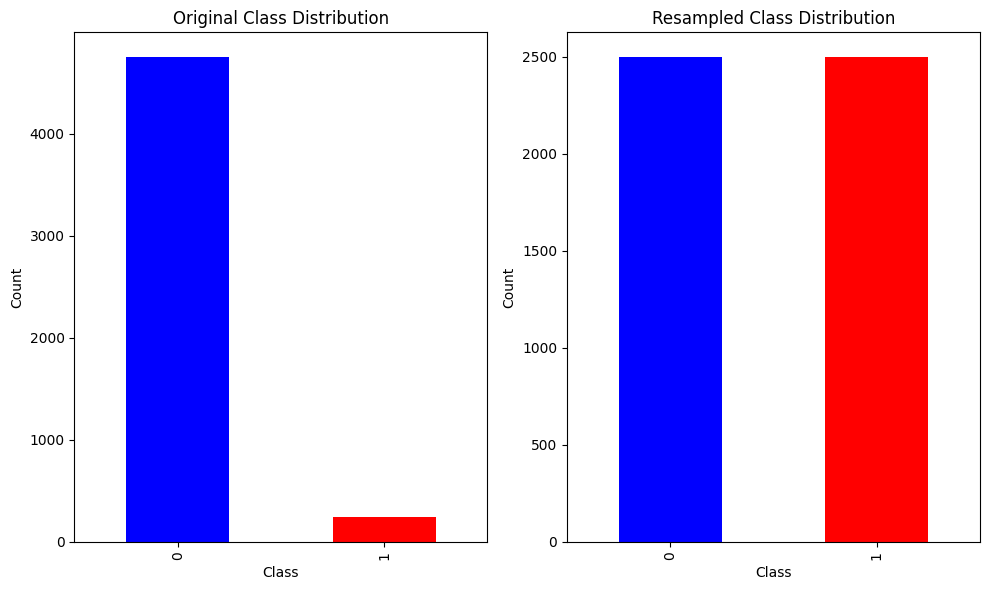
\includegraphics[width=0.95\linewidth]{images/resamp.png}}
\caption{Class Distributions}
\label{fig:resamp}
\end{figure}

\section{Results and Discussion}
\label{sec:Results-and-Discussion}

The pipeline is tested in the SensorNetGuard dataset \cite{b3}. Based on Algorithm \ref{model_select_algo}, the Extra Trees model is selected as the best performing model due to its superior metrics and efficiency. The model was then serialized as best\_model.pkl for the prediction job. 

\subsection{Exploratory Data Analysis on SensorNetGuard}
The data set SensorNetGuard is a dataset for identifying malicious sensor nodes comprising 10,000 samples with 21 features. It is designed to facilitate the identification of malicious sensor nodes in a network environment, specifically focusing on IoT-based sensor networks. The dataset includes a diverse range of features that allow for the application of machine learning models to identify various types of attacks, such as black hole, gray hole, flooding attacks, and Sybil attacks.
After dropping a few nonrelevant columns, with the remaining columns, a density plot with the remaining columns is plotted, to visualize the distribution of the data. The same is shown in Fig. \ref{fig:Distplot}. 

\begin{figure}[H]
\centerline{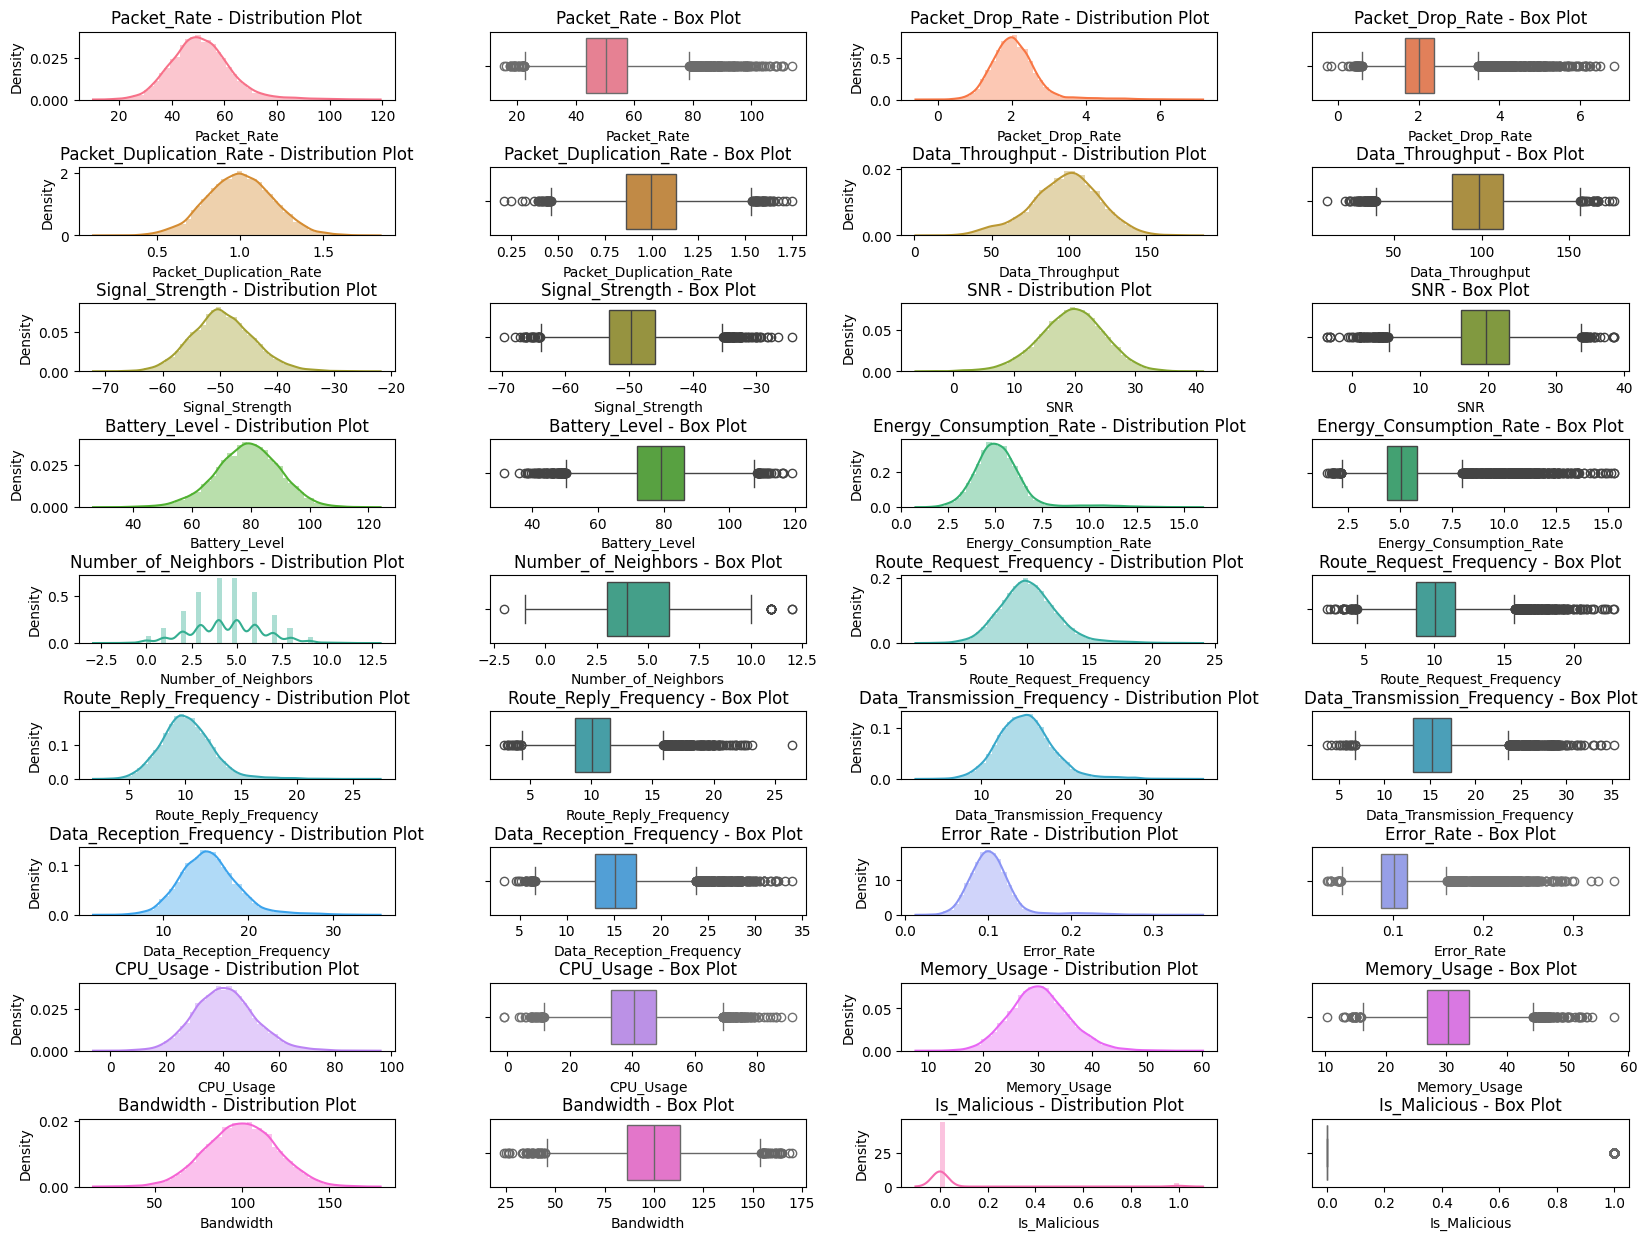
\includegraphics[width=0.95\linewidth]{images/download.png}}
\caption{Distribution Plot of the Dataset}
\label{fig:Distplot}
\end{figure}

%to be discused%
The features that exhibit the highest percentage of outliers are $Is_Malicious$ (4.87\%) and $Energy_Consumption_Rate$ (4.47\%), suggesting possible problems with power and security. Significant variability is also shown by Packet Drop Rate (3.68\%) and Error Rate (4.42\%), which may have an effect on the network's dependability. The outlier proportions for the majority of other indicators range from 1\% to 2\%, indicating periodic aberrations but overall consistency in those areas. The two metrics with the fewest outliers are Bandwidth (0.67\%) and Number of Neighbors (0.13\%), indicating more consistent behavior in these areas.The observed outliers comprise malicious nodes.

\subsection{Evaluation}
The performance of the five machine learning models is evaluated and ranked based on accuracy, precision, recall, F1 score, and training time, as shown in Table \ref{ranked_model_metrics}. The Extra Trees model achieved the highest rankings across all metrics, including accuracy (0.9994), precision (0.9994), recall (0.9994), and F1 score (0.9994), with the shortest training time of 2.25 seconds. It is worth noting that, even though LightGBM and XGBoost rank higher due to better Accuracy, Precision, Recall, F1 Score; both these models take significantly longer to train (58-59 seconds) as compared to Gradient Boosting and Random Forest.

\begin{table}[htbp]
\centering
\caption{Ranked Models with Metrics}
\resizebox{\columnwidth}{!}{
\begin{tabular}{|c|c|c|c|c|c|c|}
\hline
\textbf{Rank} & \textbf{Model} & \textbf{Accuracy} & \textbf{Precision} & \textbf{Recall} & \textbf{F1 Score} & \textbf{Training Time} \\
\hline
1 & ExtraTrees & 0.9994 & 0.9994 & 0.9994 & 0.9994 & 2.2492 \\
\hline
2 & LightGBM & 0.9984 & 0.9984 & 0.9984 & 0.9984 & 58.3919 \\
\hline
3 & XGBoost & 0.9982 & 0.9982 & 0.9982 & 0.9982 & 24.2645 \\
\hline
4 & GradientBoosting & 0.9974 & 0.9974 & 0.9974 & 0.9974 & 4.7614 \\
\hline
5 & RandomForest & 0.9970 & 0.9970 & 0.9970 & 0.9970 & 4.1090 \\
\hline
\end{tabular}
}
\label{ranked_model_metrics}
\end{table}

\begin{figure}[ht]
    \centering
    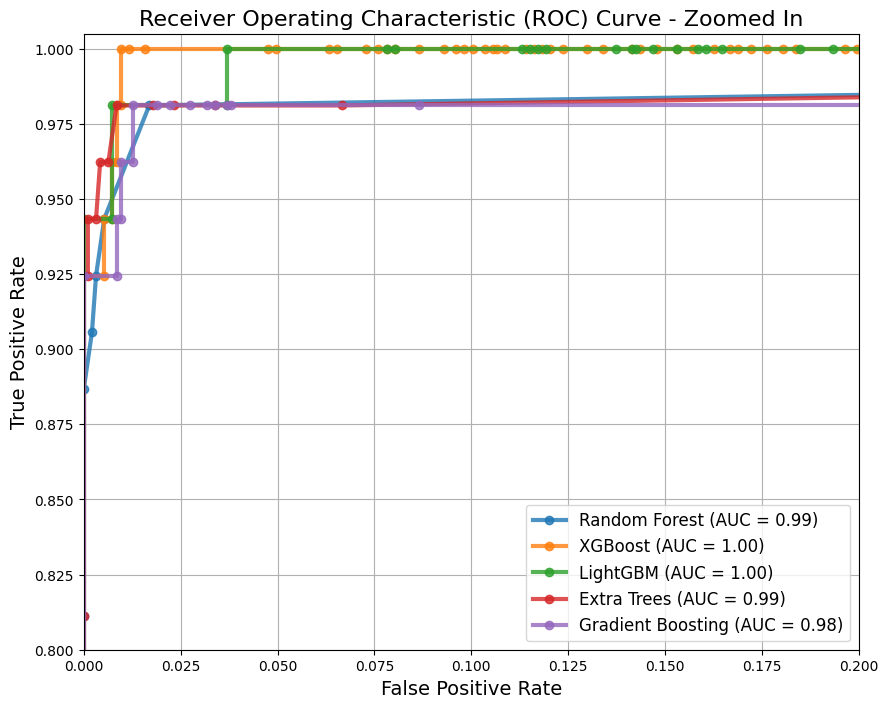
\includegraphics[width=0.85\linewidth]{images/ROC_curve.png}
    \caption{ROC Curve of Models}
    \label{fig:roc_curve}
\end{figure}

ROC Curve of the models can be seen in Fig. \ref{fig:roc_curve}. All models perform exceptionally well, with AUC values close to or at 1.00. XGBoost and LightGBM are the best-performing models while Random Forest, Extra Trees, and Gradient Boosting show a slight deviation from a perfect score.

The top 2 models are compared in figure \ref{fig:top2comp}.
\begin{figure}[ht]
\centerline{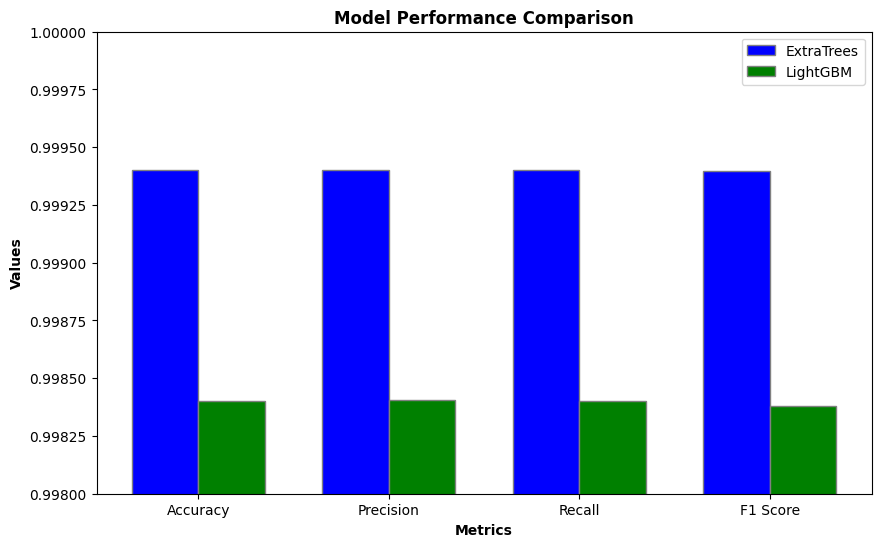
\includegraphics[width=\linewidth]{images/top2compg.png}}
\caption{Comparison of 2 best performing models}
\label{fig:top2comp}
\end{figure}

However, the main difference is depicted in figure \ref{fig:top2comptime} in terms of training time.

\begin{figure}[ht]
\centerline{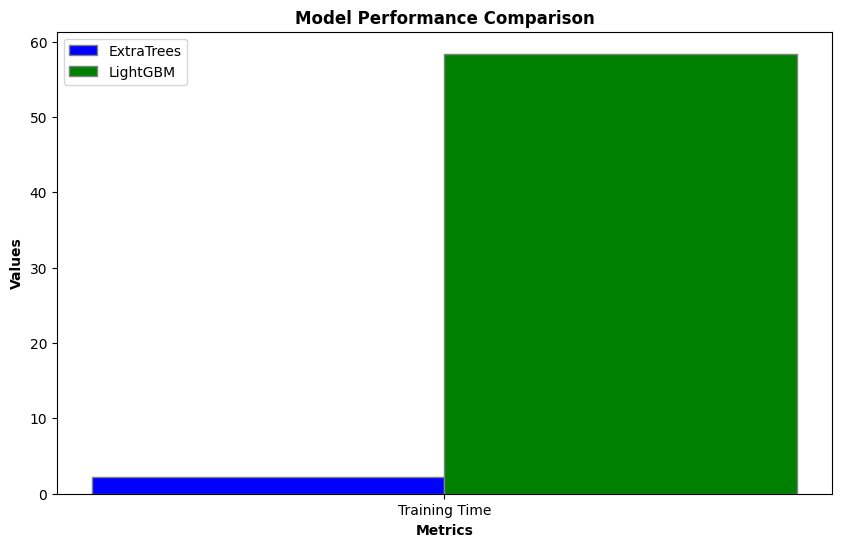
\includegraphics[width=\linewidth]{images/top2comptime.png}}
\caption{Training Time Comparison of 2 best performing models}
\label{fig:top2comptime}
\end{figure}

ExtraTrees consistently outperforms LightGBM across all metrics, though the differences are minimal. The close values indicate that both models are highly effective for the task, but ExtraTrees has a slight edge in terms of predictive performance.

To ensure robustness, 5-fold cross-validation was performed for each model. % The results are presented in Tables \ref{extratrees_fold_metrics_fold_5} through \ref{randomforest_fold_metrics_fold_}. 
The Extra Trees model consistently demonstrated high accuracy, precision, recall, and F1 scores across all folds, with only minor variations. In particular, the Extra Trees model achieved a perfect score of 1.0 in several places, reinforcing its superior performance.

LightGBM exhibited variability in its cross-validation results, with a peak accuracy of 1.0 in some cases but lower values in others, reflecting some instability. Similarly, XGBoost and Gradient Boosting showed strong results with occasional slight dips, while Random Forest displayed the most variability in accuracy and other metrics across folds.

% % Table generated by Excel2LaTeX from sheet 'extratrees_fold_metrics_fold_5'
% \begin{table}[htbp]
%   \centering
%   \caption{5 Fold Cross Validation on Extra Trees}
%     \begin{tabular}{lcccc}
%     \toprule
%     Fold  & Accuracy & Precision & Recall & F1 \\
%     \midrule
%     1     & 0.999 & 0.99900106 & 0.999 & 0.99899613 \\
%     2     & 0.999 & 0.99900105 & 0.999 & 0.99899511 \\
%     3     & 1     & 1     & 1     & 1 \\
%     4     & 1     & 1     & 1     & 1 \\
%     5     & 0.999 & 0.99900105 & 0.999 & 0.99899464 \\
%     \bottomrule
%     \end{tabular}%
%   \label{extratrees_fold_metrics_fold_5}
% \end{table}%

% % Table generated by Excel2LaTeX from sheet 'lightgbm_fold_metrics_fold_5'
% \begin{table}[htbp]
%   \centering
%   \caption{5 Fold Cross Validation on LightGBM}
%     \begin{tabular}{lcccc}
%     \toprule
%     Fold  & Accuracy & Precision & Recall & F1 \\
%     \midrule
%     1     & 0.996 & 0.99601697 & 0.996 & 0.99593645 \\
%     2     & 0.999 & 0.99900105 & 0.999 & 0.99899511 \\
%     3     & 1     & 1     & 1     & 1 \\
%     4     & 0.999 & 0.99900105 & 0.999 & 0.9989955 \\
%     5     & 0.998 & 0.99800418 & 0.998 & 0.99797832 \\
%     \bottomrule
%     \end{tabular}%
%   \label{lightgbm_fold_metrics_fold_5}
% \end{table}%

% % Table generated by Excel2LaTeX from sheet 'xgboost_fold_metrics_fold_5'
% \begin{table}[htbp]
%   \centering
%   \caption{5 Fold Cross Validation on XGBoost}
%     \begin{tabular}{lcccc}
%     \toprule
%     Fold  & Accuracy & Precision & Recall & F1 \\
%     \midrule
%     1     & 0.996 & 0.99601697 & 0.996 & 0.99593645 \\
%     2     & 1     & 1     & 1     & 1 \\
%     3     & 1     & 1     & 1     & 1 \\
%     4     & 0.998 & 0.99800421 & 0.998 & 0.99798182 \\
%     5     & 0.997 & 0.99700939 & 0.997 & 0.99695063 \\
%     \bottomrule
%     \end{tabular}%
%   \label{xgboost_fold_metrics_fold_5}
% \end{table}%

% % Table generated by Excel2LaTeX from sheet 'gradientboosting_fold_metrics_f'
% \begin{table}[htbp]
%   \centering
%   \caption{5 Fold Cross Validation on Gradient Boosting}
%     \begin{tabular}{lcccc}
%     \toprule
%     Fold  & Accuracy & Precision & Recall & F1 \\
%     \midrule
%     1     & 0.996 & 0.99601697 & 0.996 & 0.99593645 \\
%     2     & 0.995 & 0.99502615 & 0.995 & 0.99487215 \\
%     3     & 1     & 1     & 1     & 1 \\
%     4     & 0.999 & 0.99900105 & 0.999 & 0.9989955 \\
%     5     & 0.997 & 0.99700939 & 0.997 & 0.99695063 \\
%     \bottomrule
%     \end{tabular}%
%   \label{gradientboosting_fold_metrics_f}
% \end{table}%

% % Table generated by Excel2LaTeX from sheet 'randomforest_fold_metrics_fold_'
% \begin{table}[htbp]
%   \centering
%   \caption{5 Fold Cross Validation on Random Forest}
%   \resizebox{\columnwidth}{!}{
%     \begin{tabular}{lcccc}
%     \toprule
%     Fold  & Accuracy & Precision & Recall & F1 \\
%     \midrule
%     1     & 0.995 & 0.9950264830508474 & 0.995 & 0.9948998007362319 \\
%     2     & 0.994 & 0.9940376175548589 & 0.994 & 0.9938137817883511 \\
%     3     & 1     & 1     & 1     & 1 \\
%     4     & 0.999 & 0.9990010548523206 & 0.999 & 0.9989955019474808 \\
%     5     & 0.997 & 0.99700939 & 0.997 & 0.9969506281882582 \\
%     \bottomrule
%     \end{tabular}%
%     }
%   \label{randomforest_fold_metrics_fold_}
% \end{table}%

After selecting and applying the optimal model, its performance was evaluated across different window sizes to find the best evaluation threshold \cite{b17}. Testing window sizes of 500, 1000, and 2000 data points revealed that the accuracy for 1000 data points (0.968) was lower than for both 500 and 2000 data points. This suggests that training with 2000 data points offers better generalization. Additionally, Table \ref{predevalmet} shows that predictions for 2000 points are made within 5 seconds.

\begin{table}[htbp]
\centering
\caption{Performance evaluation on varying window sizes}
\resizebox{\columnwidth}{!}{
\begin{tabular}{|c|c|c|c|c|c|}
\hline
\textbf{Number of points} & \textbf{Accuracy} & \textbf{Precision} & \textbf{Recall} & \textbf{F1-Score} & \textbf{Inference Time} \\
\hline
500 & 0.988 & 0.988 & 0.988 & 0.988 & 1.25s \\
\hline
1000 & 0.968 & 0.974 & 0.968 & 0.9701 & 2.47s \\
\hline
2000 & 0.993 & 0.993 & 0.993 & 0.993 & 5.05s \\
\hline
\end{tabular}
}
\label{predevalmet}
\end{table}


% % Table generated by Excel2LaTeX from sheet 'Sheet1'
% \begin{table}[htbp]
%   \centering
%   \caption{Prediction Evaluation Metrics}
%     \begin{tabular}{ccccc}
%     \toprule
%     Number of points & Accuracy & Precision & Recall & F1-Score \\
%     \midrule
%     500 & 0.998 & 0.998 & 0.998 & 0.997 \\
%     500 & 0.988& 0.988 & 0.988 & 0.988 \\
%     1000  & 0.984 & 0.9881 & 0.984 & 0.9851 \\
%     1000  & 0.968 & 0.9746 & 0.968 & 0.9701 \\
%     1000  & 0.986 & 0.9884 & 0.986 & 0.9867 \\
%     2000 & 0.997 & 0.997 & 0.997 & 0.997 \\
%     2000 & 0.993 & 0.993 & 0.993 & 0.993 \\
     
%     \bottomrule
%     \end{tabular}%
%   \label{predevalmet}
% \end{table}%

% PLot of prediction metrics eval
% \begin{figure}[H]
%     \centering
%     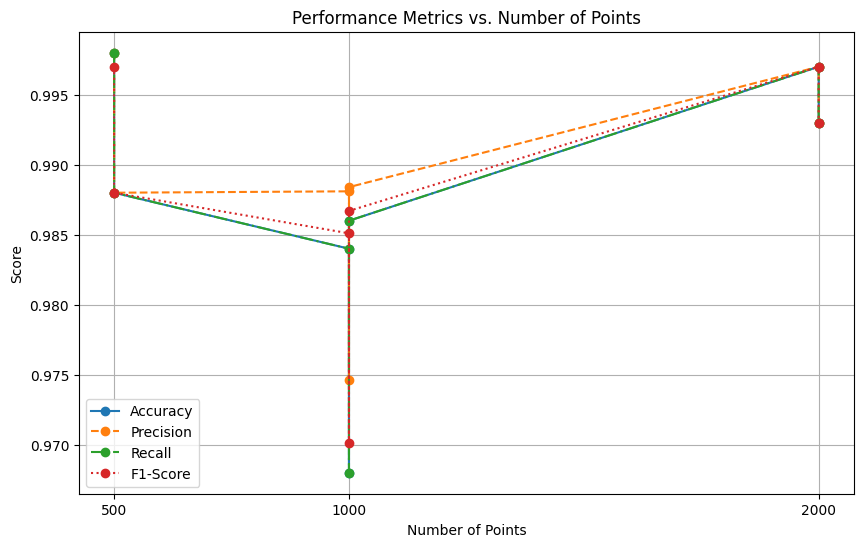
\includegraphics[width=0.85\linewidth]{images/prediction_metric_eval.png}
%     \caption{Prediction Metrics Evaluation Plot}
%     \label{fig:enter-label}
% \end{figure}

\section{Conclusion and Future Scope}
\label{sec:Conclusion-and-FutureScope}
In this paper, the researchers have developed and implemented the BARS architecture. The BARS architecture has been designed for stream-based IoT applications, incorporating multiple deep learning-driven feature selection techniques, various machine learning classifiers, race condition-based feature selection methods, and algorithmic classifier selection to enable real-time predictions with almost zero latency. This architecture conducts feature selection and model training in batch mode from data streams and subsequently makes real-time predictions in stream mode. It also assesses its predictions in a windowed manner to ensure robustness. While Kafka serves as the core of the pipeline, PostgreSQL acts as a backup in case of failure. The architecture has been deployed on the SensorNetGuard dataset to highlight its practical viability. The entire application is containerized using Docker, making it simple to relocate and deploy this pipeline on another host machine or cloud environment. An advantage of using the BARS architecture is the lower computation cost and the ability to predict in real time with minimal deployment time, along with the flexibility to customize the algorithms for feature selection, training, and prediction. Future work can focus on scalability by introducing single/multi-broker setups and multiple worker nodes for Flink and Kafka. Due to the use of Docker, transitioning to Docker Swarm or Kubernetes to add scalability in the future is quite straightforward.


%\begin{credits}
%\subsubsection{\ackname} The authors thank Center of Excellence in Internet of Things, VITAP University, for providing technical support for this work.

%\end{credits}
%
% ---- Bibliography ----
%
% BibTeX users should specify bibliography style 'splncs04'.
% References will then be sorted and formatted in the correct style.
%
% \bibliographystyle{splncs04}
% \bibliography{mybibliography}
%
\begin{thebibliography}{8}

\bibitem{b1} N. Abedzadeh and M. Jacobs, ``A Reinforcement Learning Framework with Oversampling and Undersampling Algorithms for Intrusion Detection System,'' \textit{Applied Sciences}, vol. 13, no. 20, p. 11275, 2023, doi: 10.3390/app132011275.
\bibitem{b2} C. Surianarayanan, S. Kunasekaran, and P. R. Chelliah, ``A high-throughput architecture for anomaly detection in streaming data using machine learning algorithms,'' \textit{International Journal of Information Technology}, vol. 16, no. 1, pp. 493-506, Nov. 2023, doi: 10.1007/s41870-023-01585-0.
\bibitem{b3} Dr Karthick Raghunath K M, Dr Arvind K S, September 5, 2023, "SensorNetGuard: A Dataset for Identifying Malicious Sensor Nodes", IEEE Dataport, doi: https://dx.doi.org/10.21227/ba0m-cy61.
\bibitem{b4} I. Him. "Leveraging Artificial Intelligence and Machine Learning for Real-Time Threat Intelligence: Enhancing Incident Response Capabilities,", 2024.
\bibitem{b5} A. Mudgal, S. Bhatia, "Big Data Enabled Intrusion Detection with Honeypot Intelligence System on Apache Flink (BDE-IDHIS)," in 2023 14th International Conference on Computing Communication and Networking Technologies (ICCCNT), 2023.
\bibitem{b6} Deepthi, B., et al. "An efficient architecture for processing real-time traffic data streams using apache flink," in Multimedia Tools and Applications, vol. 83, no. 13, pp. 37369–37385, 2023.
\bibitem{b7} Oliveira, R., et al. "Parameterization and Performance Analysis of a Scalable, near Real-Time Packet Capturing Platform," in Systems, vol. 12, no. 4, pp. 126, 2024.
\bibitem{b8} Maho Kajiura, Junya Nakamura, "Practical Performance of a Distributed Processing Framework for Machine-Learning-based NIDS," 2024.
\bibitem{b9} S. Atbib, C. Saadi, H. Chaoui, "Design of A Distributed Intrusion Detection System for Streaming Data in IoT Environments," in 2023 9th International Conference on Optimization and Applications (ICOA), 2023, pp. 1-6.
\bibitem{b10} F. Jemili, R. Meddeb, O. Korbaa. "Intrusion detection based on ensemble learning for big data classification," in Cluster Computing, vol. 27, no. 3, pp. 3771–3798, 2023.
\bibitem{b11} Ashraf, S., et al. "IoT empowered smart cybersecurity framework for intrusion detection in internet of drones," in Scientific Reports, vol. 13, no. 1, 2023.
\bibitem{b12} Kiran Peddireddy. "Streamlining Enterprise Data Processing, Reporting and Realtime Alerting using Apache Kafka," in 2023 11th International Symposium on Digital Forensics and Security (ISDFS), pp. 1-4, 2023.
\bibitem{b13} Kreps, J., et al, "Kafka: A distributed messaging system for log processing," in Proceedings of the NetDB, 2011, pp. 1–7.
\bibitem{b14} Paris Carbone, undefined., et al. "Apache Flink™: Stream and Batch Processing in a Single Engine," in IEEE Data Eng. Bull., vol. 38, pp. 28-38, 2015.
\bibitem{b15} A.~Akash \emph{et al.}, ``Online battery data analytics pipeline using big data tools for electric vehicles,'' in \emph{Proc. 2023 11th Int. Conf. Power Electron. ECCE Asia (ICPE 2023 - ECCE Asia)}, pp. 1207-1211, 2023.
\bibitem{b16} Bozkurt, A., Ekici, F., \& Yetiskul, H. (2023). Utilizing Flink and Kafka Technologies for Real-Time Data Processing: A Case Study. The Eurasia Proceedings of Science Technology Engineering and Mathematics, 24, 177–183.
\bibitem{b17} M.~Munir, S.~A.~Siddiqui, A.~Dengel, and S.~Ahmed, ``DeepAnT: A deep learning approach for unsupervised anomaly detection in time series,'' \emph{IEEE Access}, vol.~7, pp. 1991--2005, 2019, doi: 10.1109/ACCESS.2018.2886457.

\end{thebibliography}
\end{document}